%% This is file `elsarticle-template-1-num.tex',
%%
%% Copyright 2009 Elsevier Ltd
%%
%% This file is part of the 'Elsarticle Bundle'.
%% ---------------------------------------------
%%
%% It may be distributed under the conditions of the LaTeX Project Public
%% License, either version 1.2 of this license or (at your option) any
%% later version.  The latest version of this license is in
%%    http://www.latex-project.org/lppl.txt
%% and version 1.2 or later is part of all distributions of LaTeX
%% version 1999/12/01 or later.
%%
%% Template article for Elsevier's document class `elsarticle'
%% with numbered style bibliographic references
%%
%% $Id: elsarticle-template-1-num.tex 149 2009-10-08 05:01:15Z rishi $
%% $URL: http://lenova.river-valley.com/svn/elsbst/trunk/elsarticle-template-1-num.tex $
%%
\makeatletter
%\documentclass[12pt]{elsarticle}
\documentclass[12pt]{elsarticle}
\def\ps@pprintTitle{%
 \let\@oddhead\@empty
 \let\@evenhead\@empty
 \def\@oddfoot{}%
 \let\@evenfoot\@oddfoot}
 \makeatother
%% Use the option review to obtain double line spacing
%% \documentclass[preprint,review,12pt]{elsarticle}

%% Use the options 1p,twocolumn; 3p; 3p,twocolumn; 5p; or 5p,twocolumn
%% for a journal layout:
%% \documentclass[final,1p,times]{elsarticle}
%% \documentclass[final,1p,times,twocolumn]{elsarticle}
%% \documentclass[final,3p,times]{elsarticle}
%% \documentclass[final,3p,times,twocolumn]{elsarticle}
%% \documentclass[final,5p,times]{elsarticle}
%% \documentclass[final,5p,times,twocolumn]{elsarticle}

%% The graphicx package provides the includegraphics command.
\usepackage{graphicx}
%% The amssymb package provides various useful mathematical symbols
\usepackage{amssymb}
\usepackage{color}
\usepackage{algorithm}
\usepackage{algorithmicx}
\usepackage{algpseudocode}
\usepackage{subfigure}

%% The amsthm package provides extended theorem environments
\usepackage{amsmath}

%% The lineno packages adds line numbers. Start line numbering with
%% \begin{linenumbers}, end it with \end{linenumbers}. Or switch it on
%% for the whole article with \linenumbers after \end{frontmatter}.
%\usepackage{lineno}

%% natbib.sty is loaded by default. However, natbib options can be
%% provided with \biboptions{...} command. Following options are
%% valid:

%%   round  -  round parentheses are used (default)
%%   square -  square brackets are used   [option]
%%   curly  -  curly braces are used      {option}
%%   angle  -  angle brackets are used    <option>
%%   semicolon  -  multiple citations separated by semi-colon
%%   colon  - same as semicolon, an earlier confusion
%%   comma  -  separated by comma
%%   numbers-  selects numerical citations
%%   super  -  numerical citations as superscripts
%%   sort   -  sorts multiple citations according to order in ref. list
%%   sort&compress   -  like sort, but also compresses numerical citations
%%   compress - compresses without sorting
%%
%% \biboptions{comma,round}

% \biboptions{}

%\journal{Journal Name}

\usepackage[caption=false,font=footnotesize]{subfig}
\begin{document}

\begin{frontmatter}

%% Title, authors and addresses

\title{A Survey of Point-Based Algorithms for Solving POMDPs}

%% use the tnoteref command within \title for footnotes;
%% use the tnotetext command for the associated footnote;
%% use the fnref command within \author or \address for footnotes;
%% use the fntext command for the associated footnote;
%% use the corref command within \author for corresponding author footnotes;
%% use the cortext command for the associated footnote;
%% use the ead command for the email address,
%% and the form \ead[url] for the home page:
%%
%% \title{Title\tnoteref{label1}}
%% \tnotetext[label1]{}
%% \author{Name\corref{cor1}\fnref{label2}}
%% \ead{email address}
%% \ead[url]{home page}
%% \fntext[label2]{}
%% \cortext[cor1]{}
%% \address{Address\fnref{label3}}
%% \fntext[label3]{}


%% use optional labels to link authors explicitly to addresses:
%% \author[label1,label2]{<author name>}
%% \address[label1]{<address>}
%% \address[label2]{<address>}

\author{Andrea Bajcsy}


\begin{abstract}
%% Text of abstract
A key problem in designing autonomous systems is taking input from the environment and producing actions that allow the system to reach a goal. In most real-world settings, actions have stochastic effects on the environment and the state of the environment is only partially observable. Partially Observable Markov Decision Processes (POMDPs) are an expressive and mathematically concrete framework that enable us to optimize decision problems with partial observability. However, POMDPs are hindered by computational intractability. Thus, good approximation techniques are needed in order to leverage the modeling power of POMDPs with realistic computation.

The goal of this survey is two-fold: (1) analyze the foundations of solving POMDPs with value iteration and point-based approximations and, (2) analyze a POMDP-based model of human internal state in the context of human-robot interaction. %Analyzing some current POMDP models of human state, we show that the POMDP framework can be adapted to not only passively infer the partially observable states, but to adapt to the human user online. 
\end{abstract}

\end{frontmatter}

%\tableofcontents

%%
%% Start line numbering here if you want
%%

%% main text
\section{Introduction}
As autonomous systems begin to leave the assembly lines and actually interact with humans, there comes a need to model and predict humans actions and internal belief state in human-robot interaction settings. Partially Observable Markov Decision Processes (POMDPs) provide a solid mathematical framework for optimizing decision problems with partial observability. This is a desired characteristic in robotics applications where autonomous systems often operate under uncertain and dynamic environments. However, POMDPs are often computationally intractable, taking hours to compute an exact solution even for POMDPs with only a dozen states \cite{kurniawati2008sarsop}. This leads to POMDPs being unusable for modeling realistic robotics problems. While computing exact solutions to POMDPs remains difficult, point-based POMDP algorithms have provided fast approximate solutions for POMDPs even with hundreds of states \cite{kurniawati2008sarsop}. 


\subsection{Scope and Organization}
In order to make POMDP models usable in interactive human-robot settings, a focus on good approximations of POMDPs is worth investigation. To lay the groundwork for understanding the design and usability of POMDP models for human-robot interaction, this preliminary literature survey provides a brief overview of point-based approximations for solving POMDPs and their use in modeling spoken language interaction with model uncertainty. First, we review the fundamentals of Markove Decision Processes (MDPs) versus POMDPs. Then, we summarize the fundamental leaps in point-based value iteration algorithms for approximating discrete and continuous POMDPs. Finally, we describe the use of value iteration approximations in the context of context of an adaptive human-robot interaction system where a spoken language system must adapt to a human user. {\color{red}We find that while approximate POMDP solving methods are becoming more and more efficient, newer trends in human-robot interaction emphasize that robots can actively probe the environment in order to gather more information about the partially observable states, rather than simply relying on passive observations.}

\subsection{Background: MDPs and POMDPs}
Markov Decision Processes (MDPs) are at the base of solving complex Partially Observable Markov Decision Processes (POMDPs) and have been of interest to solving problems in robotic navigation, gesture recognition, factory control, and speech recognition systems \cite{kaelbling1998planning}, \cite{porta2006point}.

\subsubsection{Markov Decision Processes}
A MDP agent takes the state of the world as input and outputs actions that will in turn affect the state of the world. It can be described as a tuple $<S,A,T,R>$ where:
\begin{itemize}
    \item $S$: set of the world states
    \item $A$: set of actions agent can take
    \item $T$: state-transition model defined by $P(s'|s,a)$ which denotes the probability distribution of the agent ending in state $s'$, given that it was in state $s$ and took action $a$
    \item $R$: reward function defined by $R(s,a)$ which denotes the expected reward the agent gains for taking action $a$ in state $s$
\end{itemize}

It is important to note that in MDPs, the agent never has any uncertainty about it's state (although there may be uncertainty about the effects of the agent's actions on the world), and at time $t+1$, the state and reward depend only on the state and action at time $t$ (Markov Property) \cite{kaelbling1998planning}.

Typically MDP algorithms focus on finite state and action cases, but POMDPs often consider a class of MDPs with infinite state spaces. 

To act optimally, agents must maximize their long-term reward of each of their actions. Types of optimality are defined as:
\begin{itemize}
    \item finite-horizon: agent acts to maximize expected sum of reward, $R$ in the next $N$ steps: \[ E[\sum_{t=0}^{N} R_t] \]
    \item discounted infinite-horizon: agent acts to maximize sum of rewards over infinite lifetime, but discounted by geometric factor $0 < \gamma < 1$:
    \[ E[\sum_{t=0}^{\infty} \gamma^t R_t] \]
    The larger the $\gamma$ the more effect future rewards have on the current decision. 
\end{itemize}

Policies determine the behavior of an agent at any state. Policies are evaluated based on the long-run value that the agent gets from utilizing it. This evaluation comes from the value function $V(s)$ that denotes the expected sum of reward from starting at state. Below, we have summarized the typical types of policies as well as their value functions:
\begin{itemize}
    \item stationary: actions only depend on the current state and not on the time step: $\pi: S \rightarrow A$
    \begin{itemize}
        \item stationary value function: 
        \\$V(s) = R(s,\pi(s)) + \gamma \sum_{s' \in S} T(s,\pi(s),s') V(s')$
    \end{itemize}
    \item non-stationary: actions are defined as a sequence of state-to-action maps which are indexed by time: $\pi = \{\pi_t: s_t \rightarrow a_t, ~\forall~t \in T\}$
    \begin{itemize}
        \item non-stationary value function: 
        \\$V_{t}(s) = R(s,\pi_t(s)) + \gamma \sum_{s' \in S} T(s,\pi_{t}(s),s') V_{t-1}(s')$
    \end{itemize}
\end{itemize}

While there are several exact methods by which we can find the optimal policy for MDPs including policy iteration and linear programming, we will focus on value iteration and point-based approximation variants in this survey. Value iteration has been explored not only in MDPs, but also for discrete and continuous-state POMDPs, and showed promise in scaling effectively to higher dimensional states for both discrete and continuous POMDPs \cite{kaelbling1998planning}, \cite{pineau2003point}, \cite{porta2006point}. 

\subsubsection{Partially-Observable Markov Decision Processes}

In the case of POMDPs, the agent can no longer determine it's current state with complete reliability. Thus, we cannot compute the optimal policy $\pi$ and use it to act. Thus, to act truly optimally, a POMDP agent has to remember previous actions and observations to better distinguish states in it's world from previous states it has been in. 

Similarly to the MDP agent, a POMDP agent can be described as a tuple $<S,A,T,R,O,\Omega>$ where the new $O$ and $\Omega$ functions:
\begin{itemize}
    \item $T$: state-transition model defined by:
    \begin{equation}
    T(b,a,b') = P(b'|a,b) = \sum_{o \in O} P(b'|a,b,o)P(o|a,b)
    \end{equation} 
    \item $R$: reward function defined by:
    \begin{equation}
    R(b,a) =  \sum_{s \in S} b(s)r(s,a)
    \end{equation} 
    \item $O$: set of observations (providing incomplete information)
    \item $\Omega$: observation model defined by $P(o'|s,a)$ which denotes the probability distribution of the agent observing $o$ from state $s$ after having taken action $a$
\end{itemize}

In order to remember previous actions and observations, a POMDP agent keeps an internal belief state, $b(s)$ = probability of world state s, encoding this previous experience. Belief states can be represented as probability distributions over states of the world and are a sufficient statistic for the agent's history \cite{kaelbling1998planning}. In other words, if the agent computes it's current belief state then no new information about it's past states or actions would help it better understand its current state. The belief has to be updated to $b'(s)$ given an old belief $b(s)$, action $a$, and observation $o$ by:

\begin{equation}
\begin{aligned}
b'(s') = P(s'|o,a,b) = \frac{P(o|s',a)\sum_{s \in S}P(s'|a,b,s)P(s|a,b)}{P(o|a,b)} \\ = \frac{\Omega(s',a',o)\sum_{s \in S}T(s,a,s')b(s)}{P(o|a,b)}
\end{aligned}
\end{equation}

Finally, just like in MDPs, the value function for POMDPs allow us to compute an optimal policy. With value iteration we can construct the optimal non-stationary discounted value function across belief space. Let $b$ be a belief and $B$ be the set of all beliefs. Thus, the value function for a non-stationary, discrete-state POMDP can be represented as:

\begin{equation}
\label{eqn:bayes_b}
V_{t}(b) = \max_{a \in A} \{R(b,a) + \gamma \sum_{b' \in B} T(b,a,b')V_{t-1}(b') \}
\end{equation}

%In general, $t$ time-steps of an agents policy can be represented in a policy tree (see Figure \ref{fig:policy_tree} taken from \cite{kaelbling1998planning}). 

%\begin{figure}[h!]
%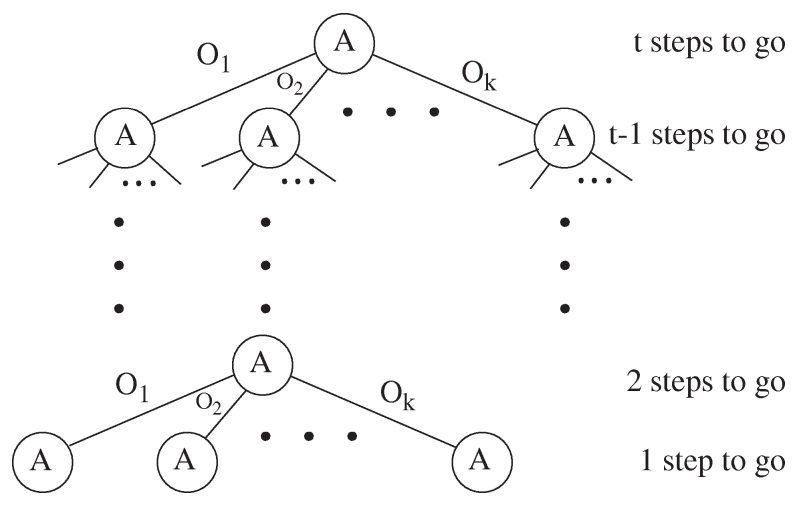
\includegraphics[width=0.6\columnwidth]{policy_tree.PNG}
%\centering
%\caption{Illustration of a POMDP policy tree. The height of the tree is the number of time steps, $t$. Each node encodes the action that should be taken given the result of the previous action.}
%\label{fig:policy_tree}
%\end{figure}

\section{Value Iteration}
\label{value_iter}
\subsection{The Value Iteration Algorithm \& Challenges}
Although value iteration was proposed in the 1970s as a method for planning in POMDPs, many POMDP value iteration algorithms aren't scalable to real-world problems \cite{pineau2003point}. Two primary reasons underlie the difficulty in scaling value iteration algorithms:
\begin{enumerate}
    \item Curse of dimensionality: If a problem has $N$ states, then belief states are in $(N-1)$ dimensional space.
    \item Curse of history: POMDP value iteration computes a set of action-observation histories, which grows exponentially with the planning horizon (think breadth-first search in belief space).  
\end{enumerate}
We can see that the higher the dimensionality of the belief space, the more action-observation histories it must compute and store. Point-based value iteration approximations seek to address the curse of history by selecting a small but representative set of belief points and applies the value iteration updates to these points. This update becomes quadratic rather than exponential which allows for greater scalability. 

The general value iteration algorithm for POMDPs can be seen in Algorithm 1. Line 5 is called the Bellman update (or Bellman back-up) and $V_{t}(b)$ represents the expected sum of rewards starting with belief $b$ and acting optimally for $H$ steps. 

\begin{algorithm}
\label{alg:VI_alg}
\begin{algorithmic}[1]
\caption{Exact Value Iteration Algorithm}
\State $V_0(s) = 0, \forall s$
\For {$t=1,2,..., H$}
    \For {$ all~s \in S$}
    \State~$V_{t+1}(b) = \max_{a \in A} \{ R(b,a) + \gamma \sum_{b' \in B} T(b,a,b')V_{t}(b')$ \}
    \EndFor
\EndFor
\end{algorithmic}
\end{algorithm}

After $H$ iterations, the solution will consist of a set of $\alpha$-vectors, each of which represent the optimal policy assuming all the following $(H-1)$ steps are optimal too. In the exact computation of the value function, it is always piecewise linear and convex in the belief \cite{kaelbling1998planning}, \cite{pineau2003point}. See Figure \ref{fig:pbvi_convex} for simple visualization of POMDP value functions. Note here that many of the computed $\alpha$-vectors have empty maximizing regions and are therefore useless in computing the optimal value function! While the pruning of such $\alpha$-vectors has been studied, it is generall expensive to identify and prune them from the set \cite{spaan2005perseus}. 

\begin{figure}[h!]
\centering 
\begin{subfigure}
    \centering 
    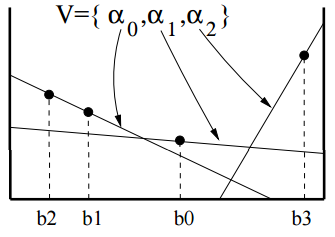
\includegraphics[width=0.4\columnwidth]{pbvi_convex.PNG}
    \centering
\end{subfigure}%
\begin{subfigure}
    \centering 
    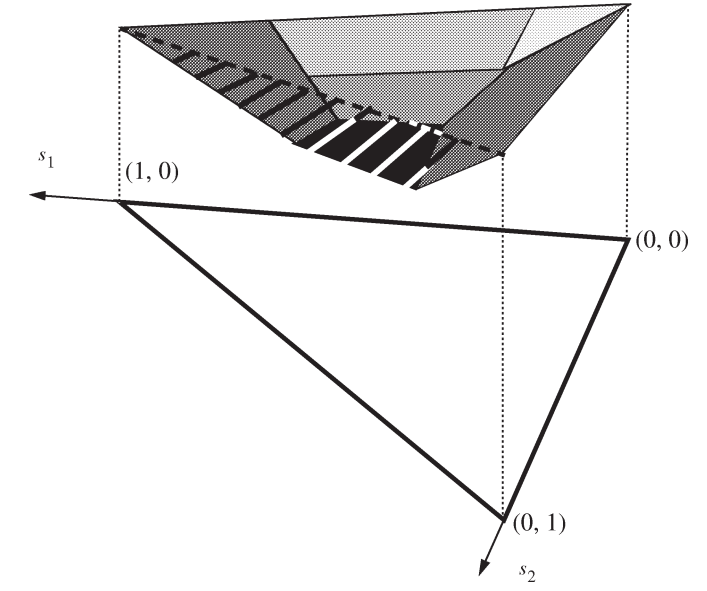
\includegraphics[width=0.4\columnwidth]{pbvi_convex3D.PNG}
    \centering
\end{subfigure}%
\caption{Illustration of 2D and 3D POMDP value functions. Each $\alpha$-vector forms a hyperplane with dimension equal to the number of states. The optimal value function takes the drawn "bowl" shape. Images from \cite{pineau2003point} (left), and \cite{kaelbling1998planning} (right).}
\label{fig:pbvi_convex}
\end{figure}

%\begin{algorithm}
%\label{alg:value_iter_alg}
%\begin{algorithmic}[1]
%\caption{Finite-State Value Iteration}
%\State $V_0(s) = 0, \forall s$
%\For {$t=1,2,...H$}
%    \For {$ all~s \in S$}
%    \State~$V_{t+1}(s) = \max_{a} \sum_{s' \in S} T(s,a,s')(V_{t}(s') + R(s,a,s'))$ 
%    \EndFor
%\EndFor
%\end{algorithmic}
%\end{algorithm}


\subsection{Point-Based Value Iteration for POMDPs}
\label{PBVI}
In \cite{pineau2003point}, the authors introduce the Point-Based Value Iteration (PBVI) algorithm for POMDP planning with a finite set of belief points. By selecting a small, representative set of belief points, this algorithm approximates the exact value iteration solution. Additionally, by using stochastic trajectories to choose belief points, PBVI is able to solve larger problems that exact value iteration methods cannot.  

The intuition behind the PBVI algorithm is that an agent should only spend time computing solutions to parts of the belief space that can actually be encountered by interacting with the environment. Thus, the PBVI algorithm starts with an initial set of belief points, $B = \{b_0, b_1, ..., b_q\}$. The algorithm initializes an $\alpha$-vector for each belief point and uses a modified version of the Bellman update to update the value of the $\alpha$-vector. Note, since PBVI preserves the full $\alpha$-vector, it ensures that the properties of piecewise linearity and convexity are preserved. The algorithm then grows the set of belief points, finds a solution, and repeats. Two questions remain: (1) how to select belief points, and (2) how to perform the efficient updates.

\subsubsection{Selecting belief points}
Initially, the set $B$ contains the initial belief $b_0$. To select new belief points for any given $b$, PBVI first stochastically simulates a step forward for each available action $a \in A$ and produces $B' = \{ b_{a_0},b_{a_1},...\}$. To simulate an action $a$, the algorithm randomly samples a state $s$ from the belief distribution $b$, then samples observation according to $\Omega(s,a,o)$, and computes $b_{a}$ with the Bayesian update in Equation \ref{eqn:bayes_b}.

To determine which sampled beliefs to keep, for each $b' \in B'$, the algorithm measures the $L_1$ distance from each $b \in B$ and discards $b'$ from the set if $b' \in B$. The resulting belief points that are kept are farthest away from any points that were already in original set $B$. At each expansion step, the new belief set at most doubles in size.

\subsubsection{Efficient point-based value updates}
The traditional Bellman update in Algorithm 1 is modified such that only one $\alpha$-vector is kept for each belief point. Due to this, the PBVI algorithm only considers beliefs that maximize the value function for at least one of the examples, visually demonstrated in Figure \ref{fig:pbvi_vs_value}.

\begin{figure}[h!]
\centering 
\begin{subfigure}
    \centering 
    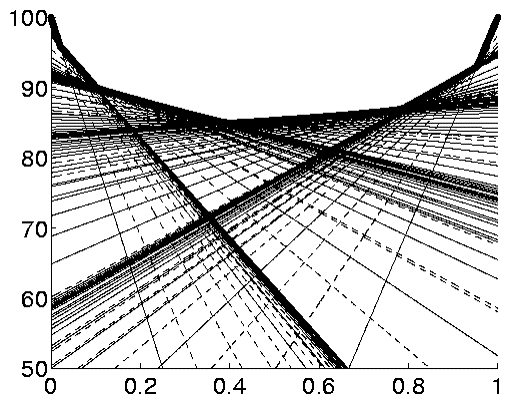
\includegraphics[width=0.4\columnwidth]{value_function.png}
    \centering
\end{subfigure}%
\begin{subfigure}
    \centering
    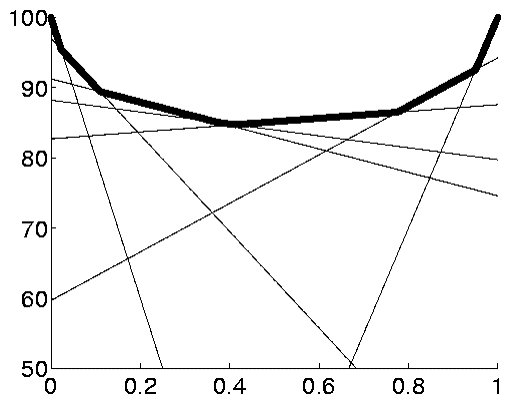
\includegraphics[width=0.4\columnwidth]{pbvi_value_function.png}
    \centering
\end{subfigure}%
\caption{Comparison of exact value function computation (left) in 2D vs. point-based value iteration computation (right). Images from \cite{weld_2012}.}
\label{fig:pbvi_vs_value}
\end{figure}

\section{Randomized Point-Based Value Iteration For POMDPs}
In \cite{spaan2005perseus}, the authors extended the original idea of point-based value iteration approximation of POMDPs from \cite{pineau2003point} to enable only updating a randomly selected subset of points in the belief set. Additionally, they show extensions from discrete action spaces to continuous action spaces as well as experimental results in large scale POMDP problems. 

The PERSEUS algorithm presented in \cite{spaan2005perseus} follows a similar paradigm as the original PBVI paper but only a random subset of belief points get updated. The claim is that a single update can ultimately improve many points in the belief set. 

\section{Application: Spoken Language Human-Robot Interaction System Modeled as POMDP}
\cite{doshi2008spoken}

\section{Discussion}

% high level comparison of the two algorithms

% they do different things, how we could apply both of them in conjunction to solve our problem
\section{Conclusion}
% what did this report do

% how does statistical learning theory help us do things/ understand things

% something about how statistical learning methods allow us to reason about complex tasks in diverse ways; the same seedling thought of choosing data effectively at each step can be used to very different ends by using interesting statistical methods.... 

\pagebreak
\section*{References}
\bibliographystyle{acm}
\bibliography{citations} 




\end{document}

%%
%% End of file `elsarticle-template-1-num.tex'.